

\subsection{Azure Data Studio }
Azure Data Studio es una herramienta de base de datos multiplataforma para profesionales de datos que utilizan la familia de plataformas de datos en la nube y locales de Microsoft en Windows, MacOS y Linux.

\begin{center}
		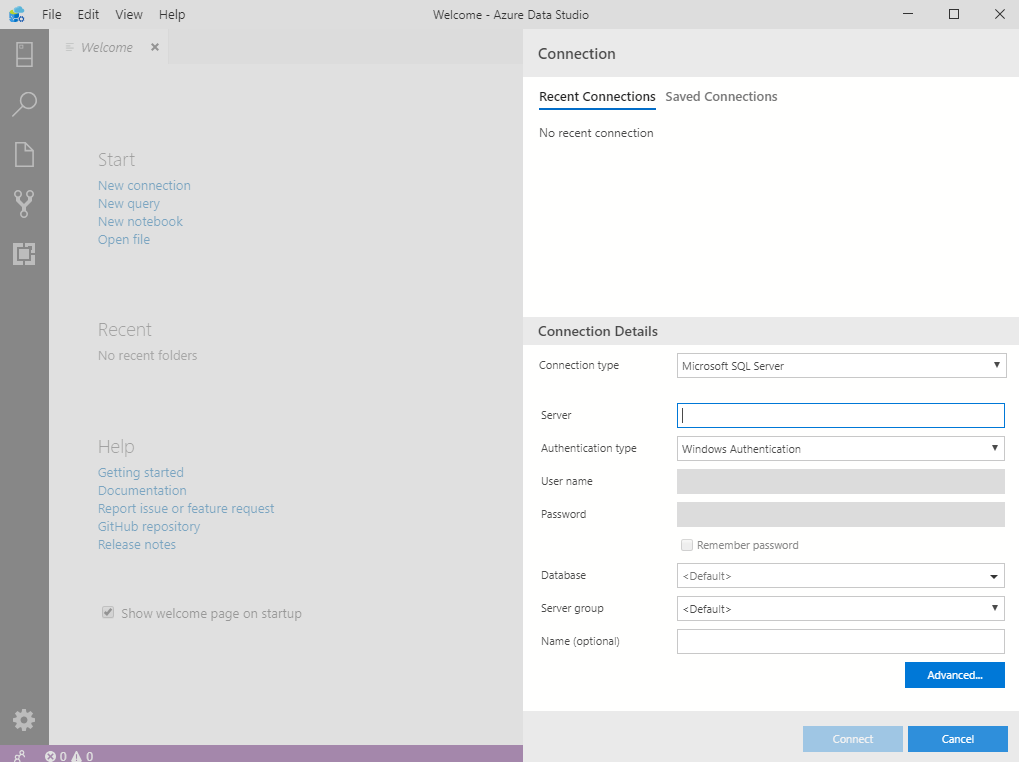
\includegraphics[width=15cm]{./Imagenes/0}
		\end{center}

\begin{center}
		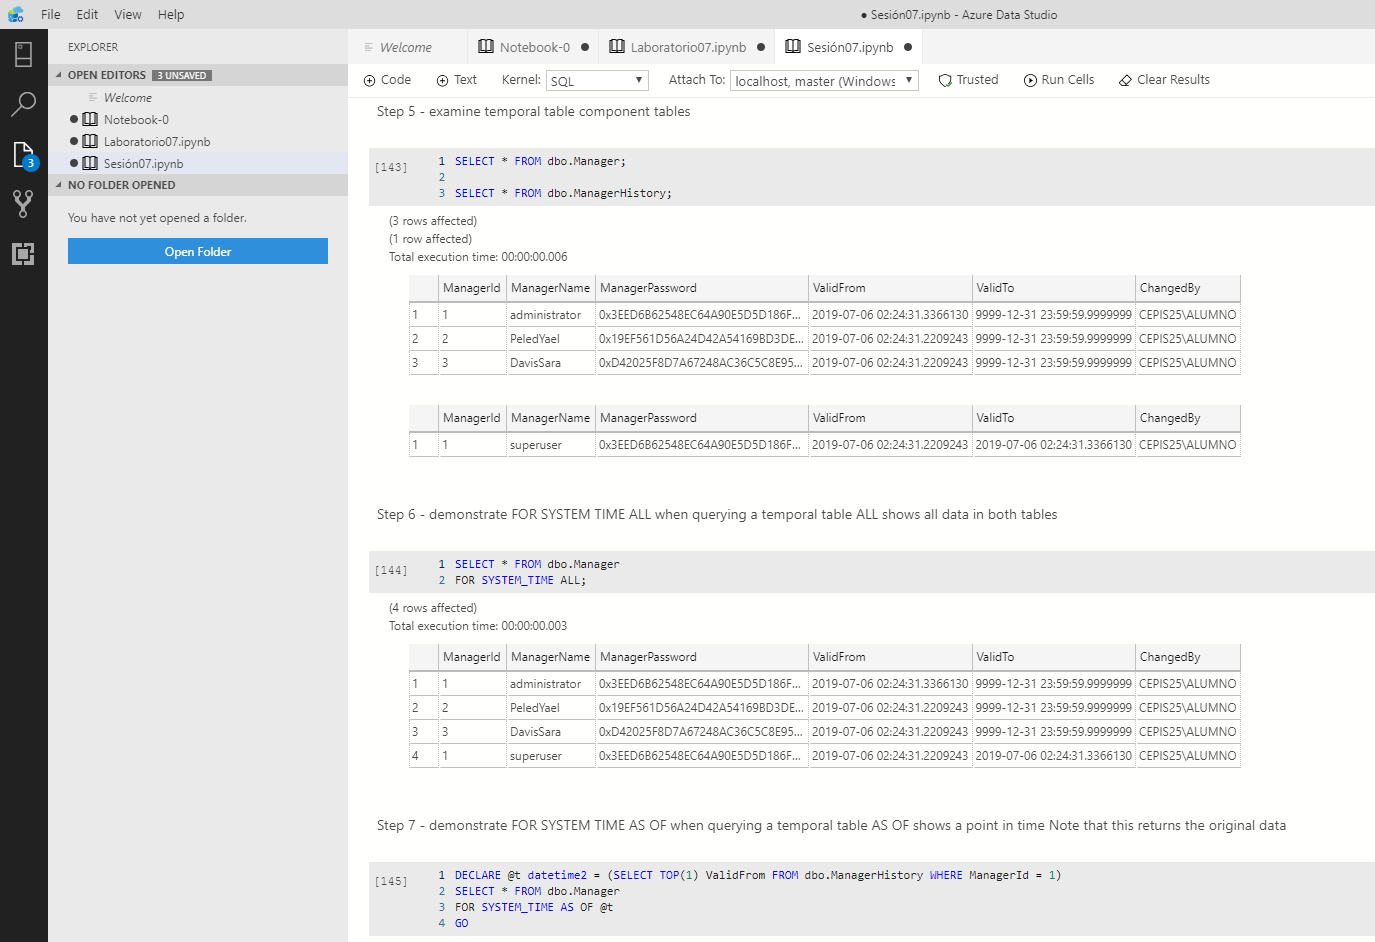
\includegraphics[width=15cm]{./Imagenes/1}
		\end{center}

\begin {itemize}
	\item Editor de código SQL con IntelliSense\\\\
	\subitem Azure Data Studio ofrece una experiencia moderna de codificación SQL centrada en el teclado que facilita sus tareas diarias con funciones integradas, como ventanas de pestañas múltiples, un editor de SQL enriquecido, IntelliSense, finalización de palabras clave, fragmentos de código, navegación de código y control de fuente integración Ejecute consultas SQL .
	\item Fragmentos de código de SQL inteligenter\\
	\subitem -Los fragmentos de código SQL generan la sintaxis SQL adecuada para crear bases de datos, tablas, vistas, procedimientos almacenados, usuarios, inicios de sesión, roles, etc., y para actualizar los objetos de base de datos existentes. Use fragmentos de código inteligente para crear rápidamente copias de su base de datos para fines de desarrollo o prueba, y para generar y ejecutar scripts CREAR e INSERTAR.\\\\
	
	\item Extensibilidad y auditoría de extensión.\\
	\subitem - Mejore la experiencia de Azure Data Studio al ampliar la funcionalidad de la instalación básica. Azure Data Studio proporciona puntos de extensibilidad para las actividades de administración de datos, así como soporte para la creación de extensiones.\\
	
\end{itemize}





